\documentclass[9pt]{beamer}
\usetheme{Antibes}
\useinnertheme{rectangles}
\useoutertheme{infolines}
\usepackage[utf8]{inputenc}
\usepackage[T1]{fontenc}
\usepackage[ngerman]{babel}

% Patch the look of +, = in arev
\usefonttheme{serif}

\usepackage{arev}
\usepackage{amsmath}
\usepackage{amssymb}

% Patch punctuation to be upright
\DeclareMathSymbol{.}{\mathpunct}{operators}{`.}
\DeclareMathSymbol{,}{\mathpunct}{operators}{`,}

\setbeamertemplate{footline}{%
\begin{beamercolorbox}[ht=3.0ex,dp=1ex]{title in head/foot}
\hfill\footnotesize\insertpagenumber\enspace\enspace\end{beamercolorbox}}

\definecolor{bluegreen1}{rgb}{0.0,0.20,0.28}
\definecolor{bluegreen2}{rgb}{0.0,0.20,0.28}
\setbeamercolor*{palette primary}{fg=white,bg=bluegreen1}
\setbeamercolor*{palette secondary}{fg=white,bg=bluegreen2}
\setbeamercolor*{palette tertiary}{fg=white,bg=bluegreen2}
\setbeamercolor{itemize item}{fg=black}
\setbeamercolor{block title}{bg=bluegreen2}
\newcommand{\modest}[1]{{\small\color{gray}#1}}

\newcommand{\ee}{\mathrm e}
\newcommand{\ui}{\mathrm i}
\newcommand{\real}{\operatorname{Re}}
\newcommand{\imag}{\operatorname{Im}}
\newcommand{\uv}[1]{\underline{#1}}
\newcommand{\bv}[1]{\mathbf{#1}}

\newcommand{\N}{\mathbb N}
\newcommand{\Z}{\mathbb Z}
\newcommand{\Q}{\mathbb Q}
\newcommand{\R}{\mathbb R}
\newcommand{\C}{\mathbb C}

\newcommand{\id}{\operatorname{id}}
\newcommand{\sgn}{\operatorname{sgn}}
\newcommand{\Abb}{\operatorname{Abb}}
\newcommand{\unit}[1]{\mathrm{#1}}
\newcommand{\chem}[1]{\mathrm{#1}}
\newcommand{\strong}[1]{\textsf{\textbf{#1}}}
\newcommand{\defiff}{\quad:\Longleftrightarrow\quad}
\renewcommand{\qedsymbol}{\ensuremath{\Box}}

\newcommand{\icol}[1]{
  \big(\!\begin{smallmatrix}#1\end{smallmatrix}\!\big)%
}

\newcommand{\parspace}{\vspace{0.8em}}


\title{Was ist eine lineare Abbildung?}
\date{}

\begin{document}

\begin{frame}
\maketitle
\end{frame}

\begin{frame}
\begin{center}
\strong{Kurze Vorbereitung}
\end{center}
\end{frame}

\begin{frame}
Unter einer Matrix versteht man eine Anordnung
\[A = \begin{pmatrix}
a_{11} & a_{12}\\
a_{21} & a_{22}
\end{pmatrix},\]
wobei die $a_{ij}$ reelle Zahlen sind.

\parspace
Die Multiplikation von $A$ mit einem Vektor
$\bv v = \icol{v_1\\ v_2}$ ist definiert als
\[A\bv v = \begin{pmatrix}
a_{11} & a_{12}\\
a_{21} & a_{22}
\end{pmatrix}\begin{pmatrix}v_1 \\ v_2\end{pmatrix}
:= \begin{pmatrix}a_{11}v_1+a_{12}v_2 \\ a_{21}v_1+a_{22}v_2\end{pmatrix}.\]
{\footnotesize{}Als Merkhilfe dient das \emph{falksche Schema}: Der
linke Zeigefinger überstreicht waagerecht die jeweilige Zeile der
Matrix, während der rechte Zeiger senkrecht den Vektor überstreicht.}
\end{frame}

\begin{frame}
\begin{center}
\strong{Rechnen mit linearen Abbildungen}
\end{center}
\end{frame}

\begin{frame}
Eine Abbildung $f\colon\R^2\to\R^2$ nennt man linear, wenn die
beiden Regeln
\begin{align*}
f(\bv a+\bv b) &= f(\bv a)+f(\bv b),\\
f(r\bv a) &= rf(\bv a)
\end{align*}
für beliebige Vektoren $\bv a,\bv b$ und eine beliebige reelle Zahl
$r$ erfüllt sind.

\parspace
Die beiden Regeln erzwingen eine große Einschränkung, welche
Gestalt eine lineare Abbildung gegenüber einer allgemeinen Abbildung
annehmen kann.
\end{frame}

\begin{frame}
Betrachten wir zunächst einen ein Vektor $\bv v = v_1\bv e_1+v_2\bv e_2$.

\parspace
Unter Anwendung der beiden Regeln erhält man\pause
\[f(\bv v) = v_1f(\bv e_1)+v_2f(\bv e_2).\]\pause
\emph{Das bedeutet aber, dass eine lineare Abbildung bereits durch ihre
Wirkung auf die Basisvektoren eindeutig bestimmt ist.}
\end{frame}

\begin{frame}
Wir definieren die Bilder als
\[\begin{pmatrix}a_{11}\\ a_{21}\end{pmatrix} := f(\bv e_1),\quad
\begin{pmatrix}a_{12}\\ a_{22}\end{pmatrix} := f(\bv e_2).\]
Dann gilt
\[f(\bv v) = v_1\begin{pmatrix}a_{11}\\ a_{21}\end{pmatrix}
+ v_2\begin{pmatrix}a_{12}\\ a_{22}\end{pmatrix}
= \begin{pmatrix}
a_{11}v_1+a_{12}v_2\\
a_{21}v_1+a_{22}v_2
\end{pmatrix}.\]\pause
Das ist die eingangs beschrieben Multiplikation einer Matrix mit einem
Vektor. Demnach ist jede lineare Abbildung von der Form
\[f(\bv v) = A\bv v,\]
wobei die Spalten von $A$ die Bilder der Basisvektoren sind.
\end{frame}

\begin{frame}
\begin{center}
\strong{Gestalt linearer Abbildungen}
\end{center}
\end{frame}

\begin{frame}
Zur Veranschaulichung einer Abbildung $f\colon\R^2\to\R^2$
betrachten wir, was $f$ mit dem Koordinatengitter macht.

\parspace
Bei einer linearen Abbildung kann das Koordinatengitter gedreht
und schiefwinklig werden, es kann auch zu einer Geraden oder einem
Punkt zusammenfallen. Die Koordinatenlinien können allerdings
niemals krummlinig werden.
\end{frame}

\begin{frame}[t]
\vspace{2em}
\begin{center}
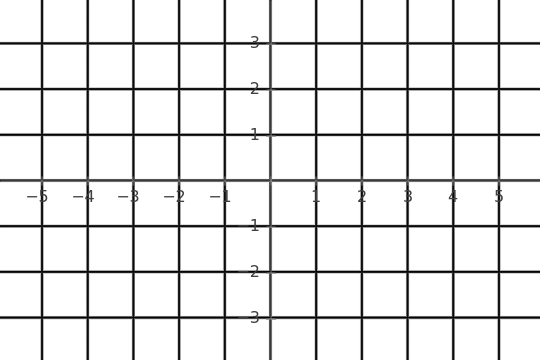
\includegraphics[width=72mm]{img/id.png}

\parspace
Die identische Abbildung $\id\icol{x\\ y}
:= \icol{x\\ y}$ lässt das\\
Koordinatengitter unberührt.
\end{center}
\end{frame}

\begin{frame}[t]
\vspace{2em}
\begin{center}
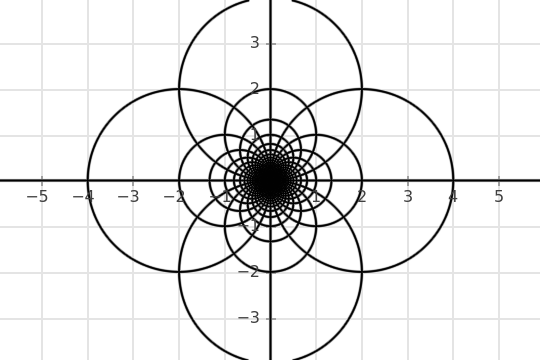
\includegraphics[width=72mm]{img/non-linear.png}

\parspace
Die Abbildung $f\icol{x\\ y}
:= \tfrac{4}{x^2+y^2}\icol{x\\ y}$
beschreibt eine Kreisspiegelung um den Kreis mit Radius zwei.
Diese nichtlineare Abbildung bewirkt krummlinige
Koordinatenlinien.
\end{center}
\end{frame}

\begin{frame}[t]
\vspace{2em}
\begin{center}
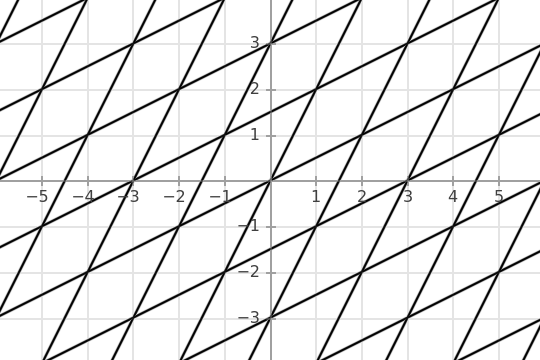
\includegraphics[width=72mm]{img/linear.png}

\parspace
Die lineare Abbildung $f\icol{x\\ y}
:= \icol{2 & 1\\ 1 & 2}\icol{x\\ y}$ bewirkt ein gedrehtes und
schiefwinkliges Koordinatengitter, wobei die Koordinatenlinien
allerdings geradlinig bleiben.
\end{center}
\end{frame}

\begin{frame}
\begin{center}
\strong{Besondere lineare Abbildungen}
\end{center}
\end{frame}

\begin{frame}
\strong{Identische Abbildung}

\parspace
Die identische Abbildung $\id(\bv v):=\bv v$ ist linear. Ihre
Matrixdarstellung ist
\[\id(\bv v) = E\bv v,\]
wobei
\[E := \begin{pmatrix}1 & 0\\ 0 & 1\end{pmatrix}\]
die \emph{Einheitsmatrix} ist.
\end{frame}

\begin{frame}
\strong{Skalierung}

\parspace
Für jede reelle Zahl $r$ ist
\[f(\bv v) := r\bv v\]
eine lineare Abbildung, die Skalierung um $r$.
\parspace

Ihre Matrixdarstellung ist
\[f(\bv v) = \begin{pmatrix}r & 0\\ 0 & r\end{pmatrix}\bv v
= rE\bv v.\]
\end{frame}

\begin{frame}
\strong{Rotation}

\parspace
Die lineare Abbildung
\[f(\bv v) := R(\varphi)\bv v\]
mit
\[R(\varphi) := \begin{pmatrix}
\cos\varphi & -\sin\varphi\\
\sin\varphi & \cos\varphi
\end{pmatrix}\]
beschreibt eine Drehung von $\bv v$ um den Winkel $\varphi$ gegen
den Uhrzeigersinn. Man nennt $R(\varphi)$ die \emph{Rotationsmatrix}
zum Winkel $\varphi$.
\end{frame}

\begin{frame}
\strong{Projektion}

\parspace
Die lineare Abbildung
\[f(\bv v) := P_{\bv u}(\bv v) =
\frac{\langle\bv u,\bv v\rangle}{\langle\bv u,\bv u\rangle}\bv u\]
beschreibt die Projektion von $\bv v$ auf die Ursprungsgerade in
Richtung des Vektors $\bv u$. Ihre Matrixdarstellung ist
\[f(\bv v) = \tfrac{1}{u_1^2+u_2^2}\begin{pmatrix}
u_1^2 & u_1 u_2\\
u_1 u_2 & u_2^2
\end{pmatrix}\bv v.\]
\end{frame}

\begin{frame}
\strong{Spiegelung}

\parspace
Die lineare Abbildung
\[f(\bv v) := S_{\bv u}(\bv v) = 2P_{\bv u}(\bv v) - \bv v\]
beschreibt eine Spiegelung an der Ursprungsgeraden in Richtung
des Vektors $\bv u$. Ihre Matrixdarstellung ist
\[f(\bv v) = \tfrac{1}{u_1^2+u_2^2}\begin{pmatrix}
u_1^2-u_2^2 & 2u_1u_2\\
2u_1u_2 & u_2^2-u_1^2
\end{pmatrix}\bv v.\]
\end{frame}

\begin{frame}
\strong{Linearform}

\parspace
Eine lineare Abbildung $f\colon\R^2\to\R$ nennt man Linearform.
Ihre Matrixdarstellung ist
\[f(\bv v) = \begin{pmatrix}a_1 & a_2\end{pmatrix}\bv v =
a_1 v_1 + a_2 v_2.\]
\end{frame}

\begin{frame}
Ende.
\vfill\hfill\modest{Juni 2021}\\
\hfill\modest{Creative Commons CC0 1.0}
\end{frame}

\end{document}

